% !TEX encoding = UTF-8
% !TEX program = xelatex
\documentclass[12pt,a4paper]{article}
\usepackage[paperwidth=210mm, paperheight=297mm, left=0.75in, right=0.75in, bottom=1in, top=1in]{geometry}
\usepackage{polyglossia}
\setdefaultlanguage[babelshorthands]{italian}
\usepackage{fontspec}
\usepackage{graphicx}
\usepackage{blindtext}
\usepackage{wrapfig}

\frenchspacing
\makeindex

\begin{document}
\title{\vspace{-70pt}Uhuru}
\author{Chiara Becchi}
\date{}
\maketitle
\pagestyle{empty}
\thispagestyle{empty}

\section*{Storia}
\label{storia}
\begin{wrapfigure}{r}{0.35\textwidth}
  \vspace{-10pt}
  \begin{center}
    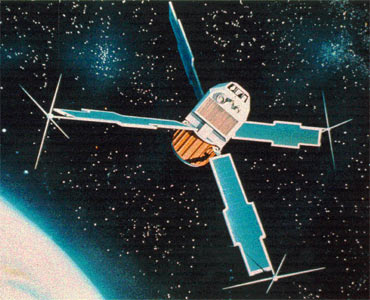
\includegraphics[width=0.30\textwidth]{satellite}
  \end{center}
  \vspace{-20pt}
\end{wrapfigure}
Uhuru è il nome del primo satellite dedicato all'astronomia a raggi X. Era anche conosciuto come X-ray explorer satellite, SAS--1, o explorer 42.
Esso fu lanciato il 12 dicembre 1970 dalla piattaforma di lancia italiana San Marco, e posto in orbita a 560 km di apogeo e 520 km di perigeo, 3 gradi di inclinazione, con un periodo di 96 minuti. La missione si completò nel marzo del 1973.

Alla realizzazione del progetto lavorarono i due scienziati italiani Riccardo Giacconi e Bruno Rossi. In particolare il ``padre'' del satellite era il fisico di origini italiane Riccardo Giacconi, emigrato negli Stati Uniti negli anni cinquanta dopo la laurea all'università di Milano. Proprio per scandagliare il cielo alla caccia di nuove sorgenti Giacconi, fisico della società di ricerca statunitense AS\&E, proponeva al centro Goddard della NASA la realizzazione di un satellite. Uhuru riusciva a disegnare la prima mappa celeste delle sorgenti X dell'universo con centinaia di emissioni misurandone intensità e variabilità nel tempo, rivelando così una dimensione del cosmo fino a quel momento sconosciuta. Altre scoperte segneranno la vita di Giacconi, che nel 2002 conquisterà il premio Nobel per la fisica. 

\section*{Osservazioni}
\label{osservazioni}

L'obiettivo della missione era scandagliare per la prima volta lo spazio alla ricerca di sorgenti di raggi X, tra cui gli ammassi di galassie, le corone stellari, le AGN (``Active Galactic Nuclei'', zone centrali di galassie particolarmente attive e luminose), alcune stelle binarie (cioè ``doppie'') ed infine eseguire, ove possibile, le osservazioni coordinate e\slash o simultanee di oggetti a raggi X con altri osservatori.

Uhuru ha raggiunto parecchi progressi scientifici tra cui la scoperta di ben 339 sorgenti X, fra queste la celebre Cygnus X--1 e Centaurus X--3; ha rivelato pulsar a raggi X e scoprì le emissioni di raggi X diffusi provenienti da ammassi di galassie, che hanno suggerito che il gas caldo può essere trovato tra le galassie. Infine ha scoperto l'esistenza dei buchi neri e ha mappato sorgenti di raggi X, come i sistemi binari stellari, resti di supernove e galassie.
L'importanza delle scoperte eseguite con questo satellite genero' il record assoluto di citazioni su pubblicazioni scientifiche.

\section*{Curiosità}
\label{curiosit}

Il nome del satellite Uhuru, nel linguaggio swahili (Africa orientale, centrale e meridionale) significa libertà. Esso fu dato in onore al popolo del Kenya che permise il lancio del satellite sul suo territorio. Inoltre l'anno del lancio, 1970, fu il settimo anniversario di indipendenza del Kenya. 


\end{document}